\documentclass[t,aspectratio=169]{beamer}
\usepackage[utf8]{inputenc}
\usepackage[T1]{fontenc}
\usepackage{xcolor}
\usepackage{hyperref}
\usepackage{tikz}
\usepackage{pgfplots}
\pgfplotsset{compat=1.8}
\usepackage{adjustbox}
\usepackage{tabularx}
\usepackage{array}
\usepackage{fontspec}
\usefonttheme{serif} % default family is serif
\usepackage{hyperref}

\title{Bayesian data analysis with TensorFlow Probability}
\date{DataScienceConference Europe 2020}
\author{Simeon Carstens \& Dorran Howell, Tweag I/O}
\newcommand{\todo}{\textcolor{red}{\textbf{TODO}}}
\renewcommand{\d}{\mathrm{d}}
\newcommand{\btVFill}{\vskip0pt plus 1filll}
\setmainfont{Roboto}
\usetheme{tweag}

\begin{document}

\begin{frame}
  \titlepage
\end{frame}


\begin{frame}
  \frametitle{Your hosts}
  \begin{tcolorbox}[title=Simeon (presentation)]
    \begin{minipage}{0.3\textwidth}{
        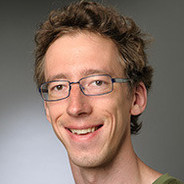
\includegraphics[width=0.15\paperwidth]{images/simeon}}
    \end{minipage}
    \begin{minipage}{0.6\textwidth}
    \begin{itemize}
    \item background in computational biology
    \item Data Scientist at Tweag since 2019
    \item lives in Paris
    \end{itemize}
    \end{minipage}
  \end{tcolorbox}

  \begin{tcolorbox}[title=Dorran (interactive demos \& questions in chat)]
    \begin{minipage}{0.3\textwidth}{
        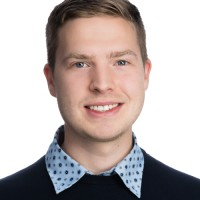
\includegraphics[width=0.15\paperwidth]{images/dorran}}
    \end{minipage}
    \begin{minipage}{0.6\textwidth}
    \begin{itemize}
    \item previous positions in geophysics
    \item Data Scientist at Tweag since 2019
    \item lives in Zurich
    \end{itemize}
    \end{minipage}
  \end{tcolorbox}
\end{frame}


\begin{frame}
  \frametitle{Tweag I/O}
  Software innovation lab and consultancy based in Paris with employees all around the world and a strong focus on open-source software.\\
  \bigskip
  We specialize in
  \begin{itemize}
  \item software engineering, with a focus on functional programming
  \item DevOps, with a focus on reproducible software systems and builds
  \item data science
  \end{itemize}
  Key industries: finance, biotech, automotive\\
  \bigskip
  Need help with your project? Want to work with us?\\
  \bigskip
  \centering
  www.tweag.io\\
  \bigskip
  hello@tweag.io
\end{frame}


\begin{frame}
  \frametitle{What you're in for}
  This tutorial consists of alternating blocks of
  \begin{itemize}
  \item theory / example slides
  \item practical examples on either external websites or Google Colab notebooks. Links at
    \begin{center}
      \url{https://github.com/tweag/tutorial-dsc-2020}
    \end{center}
  \end{itemize}

  Requirements:
  \begin{itemize}
  \item a Google account (for the hands-on demos)
  \item elementary knowledge in probability theory and statistics
  \end{itemize}
\end{frame}

\pgfmathdeclarefunction{gauss}{2}{%
  \pgfmathparse{1/(#2*sqrt(2*pi))*exp(-((x-#1)^2)/(2*#2^2))}%
}

% \tikzset{
%   normal/.pic={
%     \begin{tikzpicture}
%       \begin{axis}[
%         axis lines = left,
%         xlabel = $x$,
%         ylabel = {$p(x)$},
%         width=0.4\textwidth
%         ]
%         \addplot [
%         domain=-4:4, 
%         samples=200, 
%         color=black,
%         ]
%         {gauss(0,1)};
%       \end{axis}
%     \end{tikzpicture}
%   }
% }


% \tikzset{
%   normal_normalized_unnormalized/.pic={
%     \begin{tikzpicture}
%       \begin{axis}[
%         axis lines = left,
%         xlabel = $x$,
%         ylabel = $p(x)$,
%         xmin=-4,
%         xmax=4,
%         % TODO: ylabel not appearing
%         %width=0.4\textwidth,
%         ]
%         \addplot [
%         domain=-4:4, 
%         samples=200, 
%         color=black,
%         ]
%         {gauss(0,1)};
%         \addplot [
%         domain=-4:4, 
%         samples=200, 
%         color=black,
%         dashed
%         ]
%         {exp(-0.5*x^2)};
%         % \legend{$\mathcal{N}(x)$, $\exp(-\frac{1}{2}x^2)$};
%       \end{axis}
%     \end{tikzpicture}
%   }
% }



% \tikzset{
%   coin_prior/.pic={
%     \begin{tikzpicture}
%       \begin{axis}[
%         axis lines = left,
%         xlabel = $b$,
%         ylabel = {$p(b)$}
%         width=0.5\textwidth
%         ]
%         \addplot [
%         domain=0:1, 
%         samples=100, 
%         color=black,
%         ]
%         {x^0.5 * (1 - x)^0.5};
%       \end{axis}
%     \end{tikzpicture}
%   }
% }

% \tikzset{
%   coin_likelihood/.pic={
%     \begin{tikzpicture}
%       \begin{axis}[
%         axis lines = left,
%         xlabel = $b$,
%         ylabel = {$L(D|b)$},
%         width=0.5\textwidth
%         ]
%         \addplot [
%         domain=0:1, 
%         samples=100, 
%         color=black,
%         ]
%         {x};
%       \end{axis}
%     \end{tikzpicture} 
%   }
% }


% \tikzset{
%   coin_posterior/.pic={
%     \begin{tikzpicture}
%       \begin{axis}[
%         axis lines = left,
%         xlabel = $b$,
%         ylabel = {$p(b|D)$},
%         width=.5\textwidth
%         ]
%         \addplot [
%         domain=0:1, 
%         samples=100, 
%         color=black,
%         ]
%         {x^2 * (1 - x) * 12};
%       \end{axis}
%     \end{tikzpicture}
%   }
% }

\begin{frame}
  \frametitle{Reminder: Probabilities}
  Probability distributions can be...
  \begin{tabular}{ m{2cm} m{7cm} m{5cm}}
    discrete: & $\mathrm{Bernoulli(k; b)}=b^k(1-b)^{1-k}$ & \raisebox{-0.5\height}{\adjustbox{width=0.15\textwidth}{\includegraphics{images/bernoulli}}} \\
    continuous: & $\mathrm{\mathcal{N}(x; \mu, \sigma)}=\frac{1}{\sqrt{2 \pi \sigma^2}}\exp(-\frac{1}{2\sigma^2}(x-\mu)^2)$ & \raisebox{-0.5\height}{\adjustbox{width=0.15\textwidth}{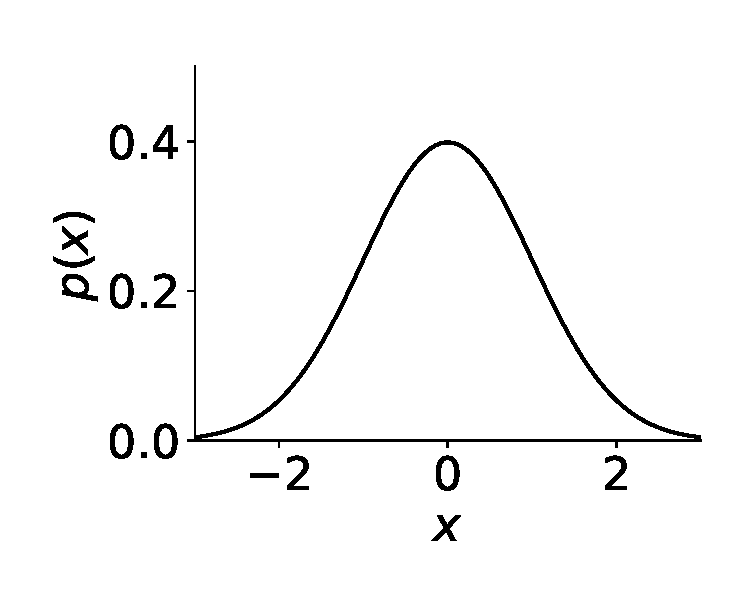
\includegraphics{images/normalized_normal}}}
  \end{tabular}\\
  Important concepts:
  \begin{description}
  \item[Conditional probability] \hfill \\ $p(A|B)$: probability that $A$ is true, given $B$ is true
  \item[Joint probability] \hfill \\  $p(A,B)$: probability that both $A$ and $B$ are true
  \item[Conditional joint probability] \hfill \\  $p(A,B|C)$: probability that both $A$ and $B$ are true, given $C$ is true
  \end{description}
\end{frame}


\begin{frame}
  \frametitle{Bayesian vs frequentist probabilities}
  Example: fair coin flip with (bias $b=\frac{1}{2}$)%$p(\mathrm{head}) = p(\mathrm{tail}) = \frac{1}{2}$
  % \begin{tcolorbox}[title=Frequentist probability]
  %   \begin{description}
  %   \item[$p(\mathrm{"flip\ results\ in\ head"}|b=\frac{1}{2})=\frac{1}{2}$:] \hfill \\ $\frac{\mathrm{\# \ of \ heads}}{\mathrm{\# \ total \ flips}}$ for $\infty$ many fair coin flips
  %   \end{description}
  % \end{tcolorbox}
  % \begin{tcolorbox}[title=Bayesian probability]
  %   \begin{description}
  %   \item[$p(\mathrm{"flip\ results\ in\ head"}|b=\frac{1}{2})=\frac{1}{2}$:] \hfill \\ measure of \textit{belief} in the statement ``flip results in head'' given single fair coin flip
  %   \end{description}
  % \end{tcolorbox}
    \begin{tcolorbox}[title=Frequentist probability]
    \begin{description}
    \item[$p(\mathrm{"head"}|b=\frac{1}{2})$:] \hfill \\ $\frac{\mathrm{\# \ of \ heads}}{\mathrm{\# \ total \ flips}}$ for $\infty$ many fair coin flips
    \end{description}
  \end{tcolorbox}
  \begin{tcolorbox}[title=Bayesian probability]
    \begin{description}
    \item[$p(\mathrm{"head"}|b=\frac{1}{2})$:] \hfill \\ measure of \textit{belief} in the statement ``flip results in head'' given a fair coin
    \end{description}
  \end{tcolorbox}
\end{frame}


\begin{frame}
  \frametitle{Prior beliefs}
  Assume: unknown bias $b$
  \begin{tcolorbox}[title=Prior probability]
    Encodes prior belief in $b$ \textit{before} flipping the coin
  \end{tcolorbox}
  \begin{columns}[onlytextwidth]
    \begin{column}{0.45\textwidth}
      What is known about $b$?
      \begin{itemize}
      \item $b$ is a probability: $0 \leq b \leq 1$
      \item most coins are fair
      \end{itemize}
      \begin{itemize}
      \item[$\rightarrow$] choose prior distribution defined between $0$ and $1$, with maximum at and symmetric around $b=\frac{1}{2}$
      \end{itemize}
      Example:
      \begin{equation*}
        b \sim \mathrm{Beta}(\alpha=2,\beta=2)
      \end{equation*}
    \end{column}
    \begin{column}[T]{0.45\textwidth}
      \begin{adjustbox}{width=\textwidth}
        \includegraphics{images/coin_flip_prior}
      \end{adjustbox}
    \end{column}
  \end{columns}
\end{frame}


\begin{frame}
  \frametitle{Posterior belief}
  Now: flip coin one time, result: $\mathrm{head}$
  \begin{tcolorbox}[title=Posterior belief]
    \begin{description}
      \item[$p(b|\mathrm{head})$:] updated prior belief after obtaining new data
    \end{description}
  \end{tcolorbox}
  \vfill
  \centering
  \adjustbox{width=0.5\textwidth}{\includegraphics{images/coin_flip_posterior}}
\end{frame}


\begin{frame}
  \frametitle{Update rule}
  \begin{tcolorbox}[title=Bayes' theorem]
    \begin{equation*}
      p(A|B) = \frac{p(B|A) \times p(A)}{p(B)}
    \end{equation*}
    (easily derived from rules for conditional probabilities)
  \end{tcolorbox}
  In data analysis:
  \begin{equation*}
    \underbrace{p(x|D,I)}_{\mathrm{posterior}} = \underbrace{p(D|x,I)}_{\mathrm{likelihood}} \times \underbrace{p(x|I)}_{\mathrm{prior}} / \underbrace{p(D|I)}_{\mathrm{evidence}}
  \end{equation*}
  \begin{description}
  \item[$x$:] model parameter (in our case: $b$)
  \item[$D$:] data (in our case: $k=1$)
  \item[$I$:] prior information (often omitted to simplify notation)
  \end{description}
\end{frame}


\begin{frame}
  \frametitle{Likelihood}
  $p(D|x)$: probability of the data given fixed model parameters\\
  $\rightarrow$ models data-generating process\\
  \bigbreak
  In our case:
  \begin{equation*}
    p(k|b) = \mathrm{Bernoulli}(k;b) = b^k(1-b)^{k-1} 
  \end{equation*}
  with
  \begin{equation*}
    k = \begin{cases} 0:& \mathrm{tail}\\
      1:& \mathrm{head}
    \end{cases}
  \end{equation*}
  \vfill
  \centering
  \adjustbox{width=0.3\textwidth}{\includegraphics{images/coin_flip_likelihood}}
\end{frame}


\begin{frame}[label=evidence_frame]
  \frametitle{Evidence}
  \onslide<1->
  \begin{description}
  \item[$p(D) = \int \d x\ p(D|x)p(x)$:]\hfill \\
    normalization constant (long story...)
  \end{description}
  In our case:
   \begin{tikzpicture}
     \node (content2) at (0,0) {\begin{minipage}{\paperwidth}
  \begin{align*}
    p(k=1) &= \int_0^1 \d b\ L(k=1|b) p(b) \\
           &= \int_0^1 \d b\ \left.\mathrm{Bernoulli}(k; b) \times \mathrm{Beta}(k;\alpha=2, \beta=2)\right\vert_{k=1} \\
           &= \int_0^1 \d b\ \left.b^{k}(1-b)^{k-1} \frac{b (1-b)}{\frac{\Gamma(2)\Gamma(2)}{\Gamma(4)}}\right\rvert_{k=1} \\
           &\;\;\vdots \\
           &=\frac{1}{2}
  \end{align*}\end{minipage}};
     \onslide<2->\node[align=center,red,font={\fontsize{50}{50}\bfseries}, rotate=45] at (content2.center) {YIKES};
   \end{tikzpicture}
\end{frame}


\begin{frame}
  \frametitle{Update rule}
  In our coin flip example:\\

  \begin{minipage}{0.15\textwidth}
    prior:
  \end{minipage}
  \begin{minipage}{0.4\textwidth}
    \raisebox{-2.0\height}{$\begin{aligned}
        p(b) &= \mathrm{Beta}(b; \alpha=2, \beta=2) \\
        &\propto b (1-b)
      \end{aligned}$}
  \end{minipage}
  \begin{minipage}{0.35\textwidth}
    \begin{adjustbox}{width=0.5\textwidth}
      \includegraphics{images/coin_flip_prior}
    \end{adjustbox}
  \end{minipage}
  
  \begin{minipage}{0.15\textwidth}
    likelihood:
  \end{minipage}
  \begin{minipage}{0.4\textwidth}
    \raisebox{-2.0\height}{$\begin{aligned}
      p(D|b) &= \mathrm{Bernoulli}(k=1; b) \\
             &= b
           \end{aligned}$}
  \end{minipage}
  \begin{minipage}{0.35\textwidth}
    \begin{adjustbox}{width=0.5\textwidth}
      \includegraphics{images/coin_flip_likelihood}
    \end{adjustbox}
  \end{minipage}

  \begin{minipage}{0.15\textwidth}
    posterior:
  \end{minipage}
  \begin{minipage}{0.4\textwidth}
    \raisebox{-2.25\height}{$\begin{aligned}
      p(b|D) &\propto p(D|b)\times p(b) / p(D)\\
             &=\mathrm{Beta}(b; \alpha=3, \beta=2) \\
             &\propto b^2(1-b)
    \end{aligned}$}
  \end{minipage}
  \begin{minipage}{0.35\textwidth}
    \raisebox{-1.5\height}{
      \begin{adjustbox}{width=0.5\textwidth}
        \includegraphics{images/coin_flip_posterior}
      \end{adjustbox}
    }
  \end{minipage}
\end{frame}

\begin{frame}
  \centering
  \vfill
  \Huge-- no slides for interactive stuff --
  \vfill
\end{frame}

% \againframe{evidence_frame}

% \begin{frame}
%   \frametitle{Intractable distributions}
%   In most cases: $p(D) = \mathrm{???}$\\
%   $\rightarrow$ 
% \end{frame}


\tikzset{
  every overlay node/.style={
    draw=black,fill=white,rounded corners,anchor=north west,
  },
}
% Usage:
% \tikzoverlay at (-1cm,-5cm) {content};
% or
% \tikzoverlay[text width=5cm] at (-1cm,-5cm) {content};
\def\tikzoverlay{%
   \tikz[baseline,overlay]\node[every overlay node]
}%


\begin{frame}
  \frametitle{Real-world Bayesian data analysis}
  \begin{columns}
    \begin{column}[T]{0.48\textwidth}
      In real problems: non-standard, difficult posterior distributions\\
    \end{column}
    \begin{column}[T]{0.48\textwidth}
      \includegraphics[width=0.5\textwidth]{images/2d_multimodal}
    \end{column}
  \end{columns}
  \begin{columns}
    \begin{column}{0.6\textwidth}
      \begin{tcolorbox}[title=Probabilistic programming libraries]
        Allow to
        \begin{itemize}
        \item programmatically define a statistical model
        \item sample from arbitrary posterior distributions
        \item run quality checks
        \end{itemize}
      \end{tcolorbox}
    \end{column}
    \begin{column}{0.38\textwidth}
      \vfill
      Examples:
      \begin{itemize}
      \item PyMC3
      \item Stan
      \item TensorFlow Probability
      \item ...
      \end{itemize}
      \vfill
    \end{column}
  \end{columns}
\end{frame}


\begin{frame}
  \frametitle{Real-world Bayesian data analysis: recipe}
  Steps to solve real-world problems:
  \begin{enumerate}
    \setcounter{enumi}{-1}
    \item Look at and think about data:
      \begin{itemize}
      \item What kind of process generated data?
      \item What do I want to learn: clusters? Approximating function? class labels?
      \end{itemize}
    \item formulate likelihood (statistical model for data-generating process)
    \item formulate prior distributions for likelihood parameters
    \item set up model in probabilistic programming library
    \item sample from posterior distribution
    \item perform quality checks
  \end{enumerate}
\end{frame}


\begin{frame}
  \frametitle{Step 0: formulating the problem and understanding the data}
  \begin{center}
    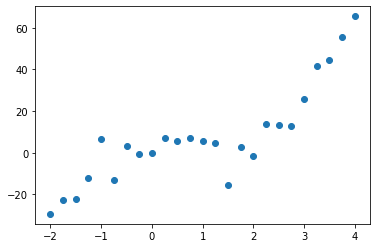
\includegraphics[width=0.7\textwidth]{images/polyfit_data.png}
  \end{center}
  \pause
  Let's do polynomial regression!
\end{frame}


\begin{frame}
  \frametitle{Step 1: formulating the likelihood}
  % \begin{columns}
  %   \begin{column}[T]{0.35\textwidth}
  \begin{center}
    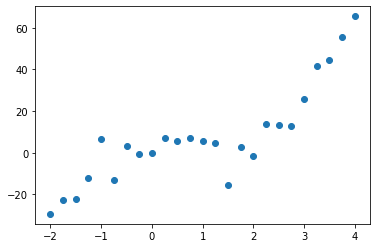
\includegraphics[width=0.5\textwidth]{images/polyfit_data.png}
  \end{center}
  %   \end{column}
  %   \begin{column}[T]{0.6\textwidth}
  %     Standard distributions generate certain types of data:
  %     \begin{description}
  %     \item[Poisson distribution:] counts per interval
  %     \item[Exponential distribution:] interarrival times
  %     \item[...]
  %     \end{description}
  %   \end{column}
  % \end{columns}
  Often: measured data = idealized data + noise\\
  \bigskip
  \begin{description}
  \item[idealized data:] $\hat f(x)=\beta_0 + \beta_1x + \beta_2x^2 + \beta_3x^3$
  \item[\phantom{zed data}noise:] normally distributed
  \end{description}
  Likelihood parameters: $\vec{\beta},\sigma$
\end{frame}

%% https://tex.stackexchange.com/a/279455
\newcommand{\shrug}[1][]{%
\begin{tikzpicture}[baseline,x=0.8\ht\strutbox,y=0.8\ht\strutbox,line width=0.125ex,#1]
\def\arm{(-2.5,0.95) to (-2,0.95) (-1.9,1) to (-1.5,0) (-1.35,0) to (-0.8,0)};
\draw \arm;
\draw[xscale=-1] \arm;
\def\headpart{(0.6,0) arc[start angle=-40, end angle=40,x radius=0.6,y radius=0.8]};
\draw \headpart;
\draw[xscale=-1] \headpart;
\def\eye{(-0.075,0.15) .. controls (0.02,0) .. (0.075,-0.15)};
\draw[shift={(-0.3,0.8)}] \eye;
\draw[shift={(0,0.85)}] \eye;
% draw mouth
\draw (-0.1,0.2) to [out=15,in=-100] (0.4,0.95); 
\end{tikzpicture}}

\begin{frame}
  \frametitle{Step 2: formulating prior distributions}
  \begin{columns}
    \begin{column}[T]{0.55\textwidth}
      \begin{tcolorbox}[title=Incorporate all available information]
        \begin{itemize}
        \item previous experiments
        \item ballpark  estimation from the data
        \item common sense
        \end{itemize}
      \end{tcolorbox}
    \end{column}
    \begin{column}[T]{0.4\textwidth}
      \begin{tcolorbox}[fontupper=\small,title=\textcolor{red}{Warning}]
        Avoid introducing strong bias!
      \end{tcolorbox}
    \end{column}
  \end{columns}
  \vfill
  \begin{columns}
    \begin{column}{0.65\textwidth}
      Noise $\sigma$:\\
      \begin{itemize}
      \item positive quantity $\rightarrow$ $p(\sigma)$ with positive support
      \item from data: not too big
      \end{itemize}
      e.g., $\sigma \sim \mathrm{Lognormal}(\mu=2, \sigma=\frac{1}{2})$\\
    \end{column}
    \begin{column}[T]{0.3\textwidth}
      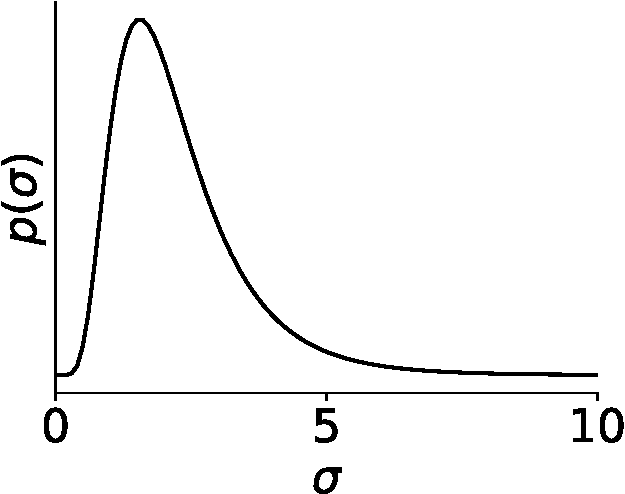
\includegraphics[width=0.7\textwidth]{images/lognormal-crop}
    \end{column}
  \end{columns}
  \begin{columns}
    \begin{column}{0.65\textwidth}
      Coefficients $\beta$:\\
      \begin{itemize}
      \item not too extreme values \shrug
      \end{itemize}
      Something broad and ``uninformative'', e.g. $\mathcal{N}(0, 5)$
    \end{column}
    \begin{column}[T]{0.3\textwidth}
      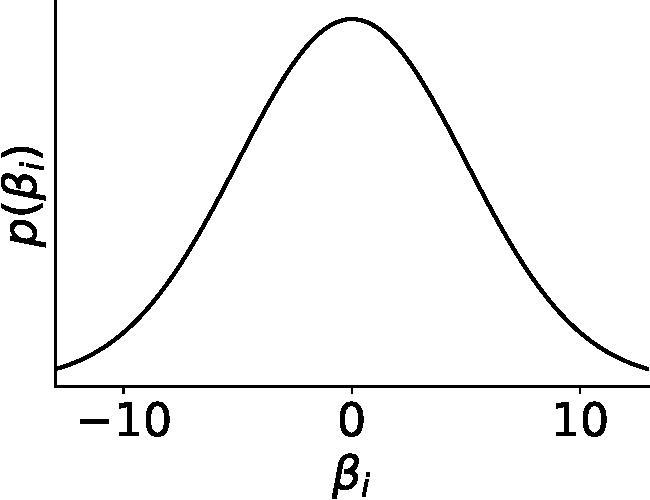
\includegraphics[width=0.7\textwidth]{images/widenormal-crop}
    \end{column}
  \end{columns}
\end{frame}

\begin{frame}
  \frametitle{Step 3: code model in probabilistic programming library}
  \centering
  \vfill
  \Huge-- see interactive demo --
  \vfill
\end{frame}

\begin{frame}
  \frametitle{Step 4: sample with appropriate inference algorithm}
  Most popular and powerful class: Markov chain Monte Carlo (MCMC)
  \begin{description}
  \item[Continuous parameters:] \hfill \\
    Hamiltonian Monte Carlo (HMC) very efficient
  \item[Discrete parameters:] \hfill \\
    e.g., Metropolis-Hastings
  \item[Combination of both:]  \hfill \\
    Gibbs sampling
  \end{description}
  Another popular option: variational inference (VI)\\
  \bigskip
  MCMC introduction blog posts:
  \begin{center}
    \url{www.tweag.io/blog}
  \end{center}
\end{frame}

% \begin{frame}
%   \frametitle{Interlude: real-world issues}
%   In reality, probability distributions often
%   \begin{itemize}
%   \item of non-standard form
%   \item are multidimensional
%   \item have highly correlated random variables
%   \item are known only up to a normalization constant
%   \end{itemize}
%   Consequences:
%   \begin{itemize}
%   \item analytical evaluation of expectation values is impossible
%   \item naïve sampling approaches are inefficient (curse of dimensionality)
%   \end{itemize}
%   \begin{columns}
%     \begin{column}[T]{0.33\textwidth}
%       \adjustbox{width=.9\textwidth}{
%         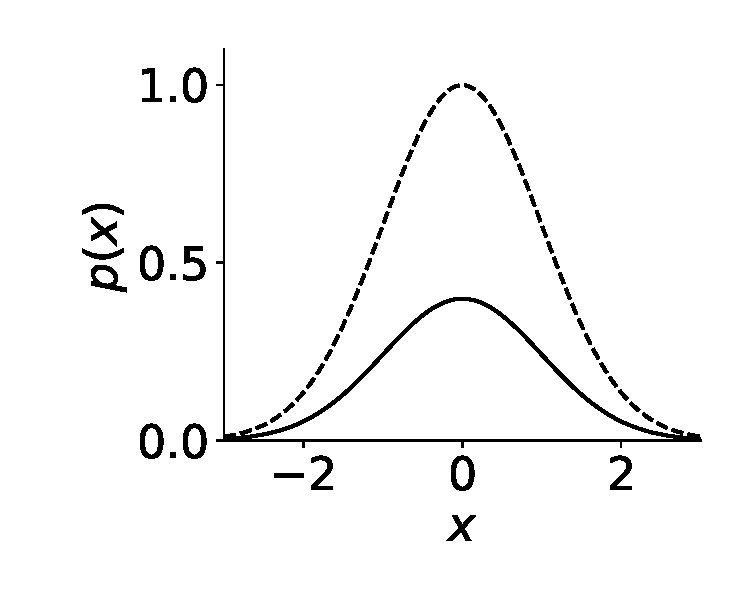
\includegraphics{images/normalized_unnormalized_normal}
%       }
%     \end{column}
%     \begin{column}[T]{0.63\textwidth}
%       \includegraphics[width=0.35\textwidth]{images/dists_multi_grid}
%       \includegraphics[width=0.35\textwidth]{images/dists_2d}
%     \end{column}
%   \end{columns}
% \end{frame}

% \begin{frame}
%   \frametitle{Real-world-ish application: regression}
%   \textbf{Step 3:} specfiy model in probabilistic programming library\\
%   \begin{itemize}
%   \item programmatic formulation of statistical model
%   \item powerful inference algorithms
%   \item ``debugging'' functionality
%   \end{itemize}
%   \bigskip\\
%   \textbf{Step 4:} perform inference with appropriate algorithm\\
% \end{frame}

\begin{frame}
  \frametitle{Approximation workhorse: Metropolis-Hastings}
  \begin{columns}
  \begin{column}{0.48\textwidth}
  \begin{tcolorbox}[fontupper=\small, title=Markov chain]
    Random process with
    \begin{equation*}
      p(x_{i+1}|x_i, x_{i-1}, \ldots, x_1) = p(x_{i+1}|x_i)
    \end{equation*}
    $\rightarrow$ a Markov chain has no ``memory''\\
    
    In some conditions: converges to a unique invariant distribution $\pi(x)$
  \end{tcolorbox}  
\end{column}
\begin{column}{0.48\textwidth}  
  \begin{tcolorbox}[fontupper=\small, title=Metropolis-Hastings algorithm]
    %\tcblower
    Construct Markov chain with invariant distribution $\pi(x)=p(x)$:
    \begin{enumerate}
    \item starting at state, $x_i$, propose a new state $x_{i+1}^*$ from $q(x_{i+1}^*|x_i)$
    \item calculate acceptance probability $p_{\mathrm{acc}}$
    \item draw $u \sim \mathcal U(0,1)$
    \item if $u < p_{\mathrm{acc}}$: $x_{i+1} = x_{i+1}^*$, else $x_{i+1} = x_i$
    \end{enumerate}
  \end{tcolorbox}
\end{column}
\end{columns}
\end{frame}


\begin{frame}{Metropolis (-Hastings)}
  Initialize with any state $x_0$\\
  \adjustbox{valign=t}{
  \begin{minipage}{0.45\linewidth}
    \par
    \noindent\phantom{\parbox{\linewidth}{%
    \begin{enumerate}
    \item calculate a proposal state $x_1^*$ by randomly perturbing $x_0$
    \item calculate acceptance probability
      \[p_\mathrm{acc}=\min\left(\frac{p(x_1^*)}{p(x_0)}, 1\right)\]
    \item with probability $p_\mathrm{acc}$, accept proposal state $x_1^*$ as the next state $x_1$, else copy $x_0$
    \end{enumerate}
    }}\par
    \vfill
    Sequence of states:\\
    $(x_0)$
  \end{minipage}}
  \hfill
  \adjustbox{valign=t}{
  \begin{minipage}{0.45\linewidth}
    \includegraphics[width=1.0\linewidth]{images/rwmc/03}
  \end{minipage}}
  \btVFill  
  \hfill \scriptsize Metropolis et al., J. Chem. Phys (1953); Hastings, Biometrika (1970)\smallskip
\end{frame}


\begin{frame}{Metropolis (-Hastings)}
  Initial state: $x_0$\\
  \adjustbox{valign=t}{
    \begin{minipage}{0.45\linewidth}
      \small
    \begin{enumerate}[<+->]
    \item calculate a proposal state $x_1^*$ by randomly perturbing $x_0$
    \item calculate acceptance probability
      \[p_\mathrm{acc}=\min\left(1, \frac{p(x_1^*)}{p(x_0)}\right)\]
    \item with probability $p_\mathrm{acc}$, accept proposal state $x_1^*$ as the next state $x_1$, else copy $x_0$
    \end{enumerate}
    \vfill
    \onslide<3>{\hbox{Sequence of states:}
      $(x_0, x_1)$}
  \end{minipage}}
  \hfill
  \adjustbox{valign=t}{
  \begin{minipage}{0.45\linewidth}
     \includegraphics<1>[width=1.0\linewidth]{images/rwmc/04}
     \includegraphics<2>[width=1.0\linewidth]{images/rwmc/05}
     \includegraphics<3>[width=1.0\linewidth]{images/rwmc/06}
  \end{minipage}}
  \btVFill  
  \hfill \scriptsize Metropolis et al., J. Chem. Phys (1953); Hastings, Biometrika (1970)\smallskip
\end{frame}


\begin{frame}{Metropolis (-Hastings)}
  Current state: $x_1$\newline
  \adjustbox{valign=t}{
    \begin{minipage}{0.48\linewidth}
      \small
    \begin{enumerate}[<+->]
    \item calculate a proposal state $x_2^*$ by randomly perturbing $x_1$
    \item calculate acceptance probability
      \[p_\mathrm{acc}=\min\left(1, \frac{p(x_2^*)}{p(x_1)}\right)\]
    \item with probability $p_\mathrm{acc}$, accept proposal state $x_2^*$ as the next state $x_2$, else copy $x_1$
    \end{enumerate}
    \vfill
    \only<3>{Sequence of states:\\
      $(x_0, x_1, x_2)$}
    \only<4>{Sequence of states:\hfill \\
      $(x_0, x_1, x_2, \ldots, x_n)$}
  \end{minipage}}
  \hfill
  \adjustbox{valign=t}{
  \begin{minipage}{0.45\linewidth}
     \includegraphics<1>[width=1.0\linewidth]{images/rwmc/07}
     \includegraphics<2>[width=1.0\linewidth]{images/rwmc/08}
     \includegraphics<3>[width=1.0\linewidth]{images/rwmc/09}
     \includegraphics<4>[width=1.0\linewidth]{images/rwmc/18}
  \end{minipage}}
  \btVFill  
  \hfill \scriptsize Metropolis et al., J. Chem. Phys (1953); Hastings, Biometrika (1970)\smallskip
\end{frame}

\begin{frame}
  \frametitle{Step 5: quality checks \& debugging}
  How to check whether sampling was successful?\\
  Effective sample size, $\hat R$ $\rightarrow$ interactive demo\\
  \bigskip
  \bigskip
  Model debugging strategy:
  \begin{columns}
    \begin{column}[T]{0.55\textwidth}
      \begin{tcolorbox}[title=Prior predictive check]
        Use prior samples to generate data points $y_k$:
        \begin{equation*}
          p(y_i) = \int \d \vec \beta \d \sigma \ L(y_k|\vec \beta, \sigma) p(\vec \beta) p(\sigma)
        \end{equation*}
      \end{tcolorbox}
    \end{column}
    \begin{column}[T]{0.4\textwidth}
      Algorithm:
      \begin{enumerate}
      \item draw samples from prior
      \item for each sample $\beta_i, \sigma_i$, you get a likelihood $L(y_k|\beta_i, \sigma_i)$
      \item draw samples from $L(y_k|\beta_i, \sigma_i)$
      \item compare if new data points $y_k$ look $\approx$ actual data
      \end{enumerate}
    \end{column}
  \end{columns}
  $\rightarrow$ interactive demo
\end{frame}
\end{document}
